% !TEX program = xelatex
% !TEX encoding = UTF-8 Unicode
% !TEX spellcheck = de_DE
% 
% © 2015–2017 Moritz Brinkmann, CC-by-sa
% http://latexkurs.github.io

\documentclass[
	vorläufig=true,
	datum=2017-12-08,
	titel={Umfangreiche Dokumente},
	web=true,
%	noshortverb=true,
	mo,
]{../tex/latexkurs-slides}

\usepackage{
	marvosym,
}

\usetikzlibrary{trees}


\begin{document}

\begin{frame}{Übersicht}
	\tableofcontents
\end{frame}

\begin{frame}{Dokumentelemente}
	\begin{itemize}
		\item Schmutztitel
		\item Titel
		\item Verzeichnisse
		\item Gliederung
		\item Kopf-/Fußzeilen
		\item Fußnoten, Randbemerkungen
		\item Formeln
		\item Abbildungen, Tabellen etc.
		\item Verweise
		\item Programmcode
		\item Anhang
		\item Bibliografie
		\item Indizes
	\end{itemize}
\end{frame}

\section{Projekte mit vielen Dateien}
\begin{frame}{Aufteilung}
	\begin{itemize}
		\item Nachteil von \TeX: lange Dokumente werden unübersichtlich\pause
		\item Vorteil von \TeX: Teile des Dokumentes können in externe Dateien ausgelagert werden
		\item geschickte Aufteilung und Verwaltung eines Dokumentes möglich
	\end{itemize}
\end{frame}

\DeleteShortVerb|

\begin{frame}{Aufteilung}
\begin{columns}
\begin{column}{.5\textwidth}
	\begin{itemize}
		\item eine Hauptdatei als leeres Gerüst
		\item eine header-Datei (evtl. weitere Datei(en) für spezielle Befehlsdefinitionen)
		\item Inhalte in einem Unterordner
		\item Abbildungen und sonstige Materialien in weiteren Unterordnern
	\end{itemize}
\end{column}
\begin{column}{.4\textwidth}
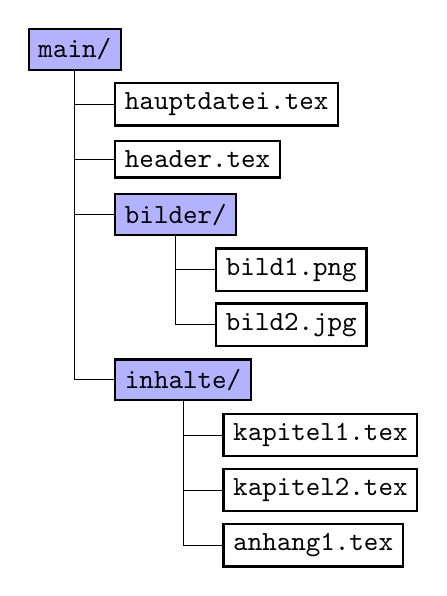
\begin{tikzpicture}[
	every node/.style={draw=black,thick,anchor=west},
	grow via three points={one child at (0.5,-0.7) and two children at (0.5,-0.7) and (0.5,-1.4)},
 	edge from parent path={(\tikzparentnode.south) |- (\tikzchildnode.west)}]
 	\ttfamily
	\node [fill=blue!30] {main/}
		child {node {hauptdatei.tex}}
		child {node {header.tex}}
%		child {node {defs}}
		child {node [fill=blue!30] {bilder/}
			child {node {bild1.png}}
			child {node {bild2.jpg}}
		}
		child [missing] {}
		child [missing] {}
		child {node [fill=blue!30] {inhalte/}
			child {node {kapitel1.tex}}
			child {node {kapitel2.tex}}
			child {node {anhang1.tex}}
		}
	;
\end{tikzpicture}
\end{column}
\end{columns}
\end{frame}
\MakeShortVerb|

\begin{frame}[fragile]{input \& include}
	\begin{itemize}
		\item |\input| und |\include| fügen externe Dateien am angegebenen Ort ein
		\item \TeX\ „springt“ aus dem aktuellen Dokument, liest woanders, und springt wieder zurück \pause
		\item \TeX-Version: |\input| liest den Code einfach ein, als gehöre er ins Hauptdokument
		\item \LaTeX-Version: |\include| erstellt eigene |.aux|-Datei (sinnvoll, wenn |.aux| benötigt)
		\item |\includeonly{a.tex,b.tex}| in der Präambel lässt nur die angegebenen Dateien für |\include| zu
		\item |\excludeonly{b.tex,c.tex}| lässt die angegebenen Dateien für |\include| \emph{nicht} zu (benötigt Paket \pkg{excludeonly})
	\end{itemize}
\end{frame}

\begin{frame}[fragile]{root-Dokument}
\begin{itemize}
	\item nach Aufteilung muss immer das Hauptdokument kompiliert werden
	\item[⇒] ständiges Wechseln zwischen Dokumenten\pause
	\item gute Editoren nehmen die Arbeit ab:
	\begin{itemize}
		\item Definition von Hauptdokumenten möglich
		\item Kompiliert automatisch das zugehörige Hauptdokument
	\end{itemize}
\end{itemize}
\pause\vfill
\begin{description}
\item[\parbox{2cm}{\vspace{-5.68cm}\flushright\TeX works\\\TeX shop\\\TeX studio}] 
Setzen von \emph{magic comments:}\\ \verb*?% !TEX root = ?\meta{Hauptdokument}
\begin{lstlisting}
% !TEX root = ../Masterarbeit.tex
% !TEX program = lualatex
% !TEX encoding = utf8
% !TEX spellcheck = de_DE
\end{lstlisting}
\item[viele IDEs] Festlegen einer „Projekt-Hauptdatei“
\end{description}
\end{frame}

\begin{frame}[fragile,t]{Beispiel-Hauptdokument}
\begin{lstlisting}
\input{header}

\includeonly{chapter1}
\excludeonly{anhang} % erfordert Paket excludeonly!

\begin{document}
  \include{chapter1}
  \include{chapter2}
   ...
  \appendix
  \include{anhang}
\end{document}
\end{lstlisting}
\vfill
⇒ Nur |chapter1| wird hier gesetzt, |anhang| explizit nie.
\end{frame}

\section{Header}
\begin{frame}[fragile]{Header-Dokument}{Einstellungen}
	\begin{itemize}
		\item Satzspiegel
		\item Schriften (Brotschrift, Überschriften)
		\item Formatierung von Formeln
		\item …
		\item alles, was vor |\begin{document}| steht
	\end{itemize}
\end{frame}

\section{Vor dem Inhalt}
\subsection{Titelei}
\begin{frame}[fragile,t]{Titelei}
	\begin{itemize}
		\item enthält alles bis zur ersten Inhaltsseite
		\item enthält Autor, Titel, etc.
		\item mit KOMA: Dokumentoption |titlepage=true/false| setzt eigene Seiten oder einen Titelkopf
		\item Umgebung |\begin{titlepage}| setzt eine frei gestaltbare Titelseite
		\item Befehl |\maketitle| setzt vordefinierte Titelei
		\item Angaben von |\title, \author, \extratitle| etc. nötig und möglich
	\end{itemize}
	\overleaf{tex0701}
\end{frame}

\begin{frame}[fragile,t]{Titeleibefehle im KOMA-Bundle}
\begin{lstlisting}
\documentclass{scrbook}
\begin{document}
  \titlehead{\Large Universität Schlauenheim}
  \subject{Masterarbeit}
  \title{Risikomanagement in Zeiten von Social Media}
  \subtitle{Design interaktiver Apps für Banken und
    Versicherungen}
  \author{cand.\,stup. Uli Ungenau}
  \date{30. Februar 2017}
  \publishers{Betreut durch Prof.\,Dr.\,rer.\,stup. Naseweis}
  \dedication{Für meine Mama.}

  \maketitle
\end{document}
\end{lstlisting}
\end{frame}

\begin{frame}[fragile,b]{|\textbackslash maketitle| (in der Beamer-Klasse)}
\begin{LTXexample}[pos=b]
\title{Risikomanagement in Zeiten von Social Media}
\subtitle{Design interaktiver Apps für Banken und
  Versicherungen}
\author{cand.\,stup. Uli Ungenau}
\date{30. Februar 2017}

\maketitle
\end{LTXexample}
\end{frame}

\begin{frame}[fragile,t]{abstract}
\begin{itemize}
	\item Umgebung |abstract| existiert für eine kurze Zusammenfassung des Dokuments
	\item mehrere Abstracts möglich (z.\,B. englisch\,/\,deutsch etc.)
\end{itemize}
\vfill
\begin{LTXexample}
\begin{abstract}
  Hier kommt eine kurze Zusammenfassung des Inhalts \dots
\end{abstract}

Und hier fängt das eigentlich Dokument an 
\dots
\end{LTXexample}
\end{frame}

\subsection{Verzeichnisse (TOC, LOF, LOT)}
\begin{frame}[fragile]{Verzeichnisse – TOC, LOF, LOT}
	\begin{itemize}
		\item Verzeichnisse fassen strukturierte Elemente zusammen
		\item prinzipiell kann alles in ein eigenes Verzeichnis aufgenommen werden
		\item übliche Verzeichnisse:
		\begin{itemize}
			\item Inhaltsverzeichnis \hfill |\tableofcontents|
			\item Abbildungsverzeichnis \hfill |\listoffigures|
			\item Tabellenverzeichnis \hfill |\listoftables|
		\end{itemize}
		\item Aufnamhme der Verzeichnisse ins Inhaltsverzeichnis: Dokumentenoption |toc=totoc|
		\item möglich: Codeverzeichnis, Beispielverzeichnis, …
	\end{itemize} 
	\overleaf{tex0701}
\end{frame}

\section{Im Inhalt}
\subsection{Fußnoten, Randbemerkungen}
\begin{frame}[fragile]{Fußnoten, Randbemerkungen}
	zusätzlicher Text, der nicht ins Hauptdokument\,/\,in den Textfluss passt
	\begin{itemize}
		\item Fußnoten \hfill |\footnote{}|
		\item gleitende Randnotiz \hfill |\marginpar|
		\item Randbemerkung  (Paket \pkg{marginnote}) \hfill |\marginnote|
	\end{itemize}
	\vfill
	Paket \pkg{footmisc} bietet vielfältige Möglichkeiten Aussehen von Fußnoten anzupassen
\end{frame}

\subsection{Zitate}
\begin{frame}[fragile]{Zitate}
Es gibt eigene Umgebungen für Zitate:
\begin{itemize}
\item |quote| für kurze Zitate
\item	 |quotation| für längere Zitate
\item |verse| für Gedichte
\end{itemize}
Das Paket \pkg{csquotes} passt Feinheiten von Anführungszeichen für den nicht-englischen Satz an.
\vfill
\begin{lstlisting}
\begin{quote}
  alea iacta est \hfill\textit{Caesar}
\end{quote}
\end{lstlisting}
\end{frame}

\subsection{Verweise}
\begin{frame}[fragile]{Verweise}
	\begin{itemize}
		\item Elemente können mittels |\label{}| bezeichnet werden
		\item mögliche Elemente sind Überschriften (sections etc.), |table|, |figure|, Formeln, …
		\item Referenzierung mit |\ref{}|
		\item Pakete liefern vielfältige Referenzierungsmöglichkeiten:\\%
		\pkg{fancyref}, \pkg{varioref}, \pkg{cleveref}\\%
		\item geschicktes Benennen:\\
		|\label{fig:Haus}| ⇒ Pakete können erkennen, dass es eine Abbildung ist
	\end{itemize}
\end{frame}

\subsection{Links}
\begin{frame}[fragile,t]{Links im Dokument}{hyperref}
\begin{itemize}
\item Paket \pkg{hyperref} macht Verweise im PDF anklickbar
\item |\ref| und |\cite| wird automatisch verlinkt
\item	 URLs können mit |\url{|\meta{URL}|}| angegeben werden
\item	 benannte Links mit |\href{|\meta{URL}|}{|\meta{angezeigter Text}|}|
\end{itemize}
\uncover<2>{Um Probleme zu vermeiden \pkg{hyperref} eher als letztes Paket laden!}
\vfill
\begin{LTXexample}
\url{http://xkcd.com}\\
\href{mailto:mo@uni-hd.de}{\huge\Letter}
\end{LTXexample}
\end{frame}


\section{Nach dem Inhalt}
\begin{frame}[fragile]{Anhang}
\begin{itemize}
\item Befehl |\appendix| schaltet auf Anhang um
\item Nummerierung startet neu\\(abhängig von Dokumentenklasse A, B, C, …)
\item Abschnitte im Anhang wie gewohnt mit |\chapter|, |\section|, etc.
\end{itemize}
\vfill
\begin{lstlisting}
\appendix
\end{lstlisting}
\end{frame}


\subsection{Bibliografie}
\begin{frame}[fragile]{Bibliografie}
\begin{itemize}
	\item Bibliografie enthält Liste verwendeter Quellen und ggf. weiterführende Literatur.
	\item je nach Fachbereich unterschiedliche Zitierstile
	\item (grobes) Aussehen der Bibliografie wird von Dokumentenklasse bestimmt.
	\item bestimmte Syntax zum Setzen der Bibliografie:
	\begin{itemize}
		\item Umbegung |\begin{thebibliography}{|\meta{Anzahl}|}|
		\item Aufzählung der Werke mittels |\bibitem{|\meta{Key}|}| \meta{Text}
		\item Zitieren eines Werks mit |\cite{|\meta{Key(s)}|}| oder |\cite[|\meta{Seite}|]{|\meta{Key}|}|
	\end{itemize}
\end{itemize}
\end{frame}


\begin{frame}[fragile,t]{Bibliografie}
\begin{lstlisting}
\begin{thebibliography}{9}
  \bibitem{frankfurt05} Harry G. Frankfurt:
    \textit{On Bullshit}, Princeton University Press,
    Princeton, New Jersey, 2005.
\end{thebibliography}
\end{lstlisting}
\vfill
\pause
\begin{itemize}
	\item manuelles Erstellen (und Sortieren) der Bibliografie ist sehr umständlich
	\item Einträge nicht sinnvoll wiederverwendbar
	\pause
	\item[⇒] Programm \BibTeX\ übernimmt Sortierung und Verwaltung der Einträge (siehe Vorlesung nach den Ferien)
\end{itemize}
\end{frame}


\subsection{Code}
\begin{frame}[fragile]{Setzen von Code}
	\begin{itemize}
		\item für kurze Sequenzen: |\verb~\befehl~|
		\item für längere Sequzenzen: |\begin{verbatim} \befehle \end{verbatim}|
		\item beide bieten |*|-Version für Anzeigen von Leerzeichen: \verb$ $
		\item Paket \pkg{listings} kann rudimentäre Syntaxhervorhebung für viele Programmiersprachen
		\item Paket \pkg{minted} nutzt externen Parser für komplexe Syntaxhervorhebung
		\item für Setzen von \LaTeX-Beispielcode: Paket \pkg{showexpl}
	\end{itemize}
\end{frame}

\subsection{Index}
\begin{frame}[fragile]{Indexerstellung}
	\begin{itemize}
		\item Indexerstellung ist immens aufwändiges Unterfangen:
		\item sämtliche (sinnvollen!) Erscheinungen von Namen\,/\,Ereignissen\,/\,Sachthemen müssen registriert werden\\%
		nicht jede Nennung eines Namens soll im Index erwähnt werden!
		\item sinnvolle Seitenangabe: 1, 2–4, 17
	\end{itemize} 
\end{frame}

\begin{frame}[fragile]{Indexerstellung}
	\begin{itemize}
		\item dank logischer Struktur leichte Erstellung in \TeX:
		\item Definieren von Befehlen erleichtert die Eingabe:\\%
			|\euler| statt | Euler \index{Euler}|
		\item mit \LaTeX\ dreistufiger Prozess:
		\begin{itemize}
			\item im \LaTeX-Lauf wird Hilfsdatei erstellt
			\item Verarbeitung mittels Programm |makeindex| (Sortierung, Seitenangaben etc.)
			\item Einbettung im nächsten \LaTeX-Lauf
		\end{itemize}
	\end{itemize}
\end{frame}

\begin{frame}[fragile,t]{Indexerstellung}{makeidx}
\begin{block}{im Dokument}
\begin{lstlisting}
\usepackage{makeidx}
\makeindex %% VOR \begin{document}!!

\index{Stichwort} %% IM Dokument!

\printindex %% druckt das Verzeichnis hier
\end{lstlisting}
\end{block}
\vfill
\begin{block}{in der Kommandozeile}
Aufruf von\\
|$ makeindex hauptdocument|\\ 
im Ordner des Hauptdokumentes
\end{block}
\end{frame}

\begin{frame}[fragile]{Indexerstellung}{multind}
\pkg{multind} ermöglicht Erstellung mehrerer Indizes – Unterscheidung mit zusätzlichem Attribut:
\begin{block}{im Dokument}
\begin{lstlisting}
\usepackage{multind}
\makeindex{stichwoerter}
\makeindex{Personen}
\index{Stichwoerter}{Stichwort}
\index{Personen}{Euler}
\printindex{stichwoerter}{Index der Stichwörter} 
\printindex{personen}{Personenverzeichnis}
\end{lstlisting}
\end{block}
\begin{block}{in der Kommandozeile}
|$ makeindex personen|\\
|$ makeindex stichwoerter|
\end{block}
\end{frame}

\begin{frame}[fragile]{Indexerstellung}{xeindex}
\begin{itemize}
\item Paket \pkg{xeindex} verwendet \hologo{XeTeX}-Interna, um automatisch Indizes zu erstellen
\item \pkg{xesearch} durchsucht dabei (mittels \hologo{XeTeX}-Befehlen!) selbst das Dokument
\item gefundene Einträge werden Indiziert\pause
\item[$+$] extrem leichtes Erstellen von Indizes beliebiger Größe
\item[$-$] Sinnhaftigkeit fragwürdig – nicht jede Nennung eines Begriffes sollte indiziert werden, sonst ist der Index nutzlos.\\
Der Leser sollte nur die wichtigsten Einträge finden.
\end{itemize}
\end{frame}

\begin{frame}[fragile]{Indexerstellung}{xeindex}
\begin{itemize}
\item verwendet intern \pkg{makeidx}, daher sind |\makeindex|, |\printindex| und |\index| weiter verfügbar
\item zu suchende Einträge:
\end{itemize}
\begin{block}{IndexList}
|\IndexList⟨*⟩{⟨name⟩}{⟨list of entries⟩}|\\
\pkg{*} ⇒ case insensitive\\
\pkg{name} ⇒ beliebiger Name für die Liste (mehrere möglich)\\
\pkg{list of entries} ⇒ |katze, hund?, maus|\\
\pkg{hund?} ⇒ findet auch |hundehütte|
\end{block}
\end{frame}


%\begin{frame}[fragile,t]{Indexerstellung}{luaindex}
%\begin{itemize}
%\item \pkg{luaindex} erlaubt es, einen Index in \hologo{LuaTeX} ohne Aufruf von externen Programmen
%\item bisher experimentelles Paket ohne Dokumentation\\
%Nutzung noch(!) nicht empfehlenswert
%\end{itemize}
%\vfill
%\begin{lstlisting}
%\makeindex
%
%\index{Indexeintrag}
%\index[sort={j}, pageformat=\emph]{Indexeintrag}
%\subindex{Indexeintrag}{Untereintrag}
%\subsubindex{Indexeintrag}{Untereintrag}{Unteruntereintrag}
%
%\printindex
%\end{lstlisting}
%\end{frame}


\section{Alternative Klassen}
\begin{frame}{Alternative Dokumentenklassen}
\begin{itemize}
\item Klasse \pkg{memoir} bietet gute Alternative für anspruchsvollen Buchsatz. 
\begin{itemize}
\item viele vordefinierte Stile. 
\item extrem anpassbar durch viele Optionen
\end{itemize}
\item Klasse \pkg{classicthesis} imitiert den Stil von Robert Bringhursts „The Elements of Typographic Style“ für Abschlussarbeiten.
\begin{itemize}
\item Hilfreiche Vorlagen erleichtern den Einstieg.
\item typografisch sehr ansprechend
\end{itemize}
\end{itemize}
\end{frame}



\nocite{dante:koma, classicthesis, memoir}
\begin{frame}[allowframebreaks]{Weiterführende Literatur}
\printbibliography
\end{frame}

\end{document}
